\documentclass[aspectratio=169, 11pt]{beamer}

\usetheme{Madrid}
\usecolortheme{whale}

\definecolor{dukeblue}{RGB}{44,62,80}
\definecolor{killred}{RGB}{192,57,43}
\definecolor{liveteal}{RGB}{22,160,133}

\setbeamercolor{structure}{fg=dukeblue}
\setbeamercolor{frametitle}{bg=dukeblue, fg=white}
\setbeamercolor{title}{bg=dukeblue, fg=white}
\setbeamercolor{subtitle}{fg=white}
\setbeamercolor{author}{fg=dukeblue}
\setbeamercolor{institute}{fg=dukeblue}
\setbeamercolor{date}{fg=dukeblue}
\setbeamercolor{palette primary}{bg=dukeblue, fg=white}
\setbeamercolor{palette secondary}{bg=dukeblue!85, fg=white}
\setbeamercolor{palette tertiary}{bg=dukeblue!70, fg=white}
\setbeamertemplate{navigation symbols}{}
\setbeamertemplate{footline}[frame number]
\setbeamertemplate{bibliography item}[text]

\usepackage{graphicx}
\usepackage{booktabs}
\usepackage{amsmath}

\newcommand{\rstar}{r^{*}}
\newcommand{\kills}{\textcolor{killred}{\textbf{dead}}}
\newcommand{\lives}{\textcolor{liveteal}{\textbf{survives}}}

\title[Fed--Market $\rstar$ Wedge]{Does the Risk Premium Move with the
Fed--Market $\rstar$ Wedge?}
\subtitle{Gate results and one honest problem}
\author{Aaron Huberman}
\institute{Duke University}
\date{10 August 2026}

\begin{document}

\begin{frame}[plain]
    \titlepage
\end{frame}

% ------------------------------------------------------------------
\begin{frame}{The question}

\textbf{The object.} Before each FOMC meeting there is a signed gap between
what the Fed says the longer-run policy rate is and what the market is
pricing: $\Delta_t = \rstar_{Fed,t} - \rstar_{Mkt,t}$.

\vspace{0.7em}

\textbf{The decomposition.} A long yield is an expectations component plus a
term premium. Hillenbrand~[2] shows the announcement window carries the entire
secular decline in yields and attributes it to the market learning the Fed's
longer-run view --- an \emph{expectations} channel. He does not decompose.

\vspace{0.7em}

\textbf{The gap.} Rungcharoenkitkul and Winkler~[1] build the two-belief
structure this question needs, simulate yield curves in Section~6, and state
in footnote~14 that the model embeds zero term premia. So the premium
component is assumed away by one paper and not measured by the other.

\vspace{0.7em}

\textbf{This talk.} Whether the \emph{premium} component of the
announcement-window move responds to the pre-meeting wedge. Everything below
is a gate result: I ran the falsification conditions before running the test.

\end{frame}

% ------------------------------------------------------------------
\begin{frame}{Construction}

\textbf{Fed side.} SEP longer-run federal funds median minus longer-run PCE,
57 dot-plot meetings, January 2012 through March 2026. Participant-level
where the compilations are de-anonymised, which is 36 meetings through 2020.

\vspace{0.6em}

\textbf{Market side, two candidates run side by side.} The Survey of Primary
Dealers longer-run funds rate, 92 surveys; and the ACM~[3] 9y1y risk-neutral
forward, $10 \cdot \text{RNY}_{10} - 9 \cdot \text{RNY}_{9}$, daily. The
second is pricing-based and has the premium already stripped.

\vspace{0.6em}

\textbf{Event panel.} 116 scheduled FOMC announcements, 2012--2026. The wedge
is measured \emph{strictly before} the announcement: the Fed side is the
\emph{previous} SEP, because the current one is released at the announcement
itself. This is the ex-ante requirement, not a robustness check --- if the
announcement closes the wedge, a contemporaneous measure is endogenous by
construction.

\vspace{0.6em}

\textbf{Window.} Two-day change, $t-1$ to $t+1$, in $y^{(n)}$, its
risk-neutral component and its term premium, $n = 1, \dots, 10$. The additive
identity holds to $1.4 \times 10^{-14}$ bp.

\end{frame}

% ------------------------------------------------------------------
\begin{frame}{The two wedges}
    \begin{center}
        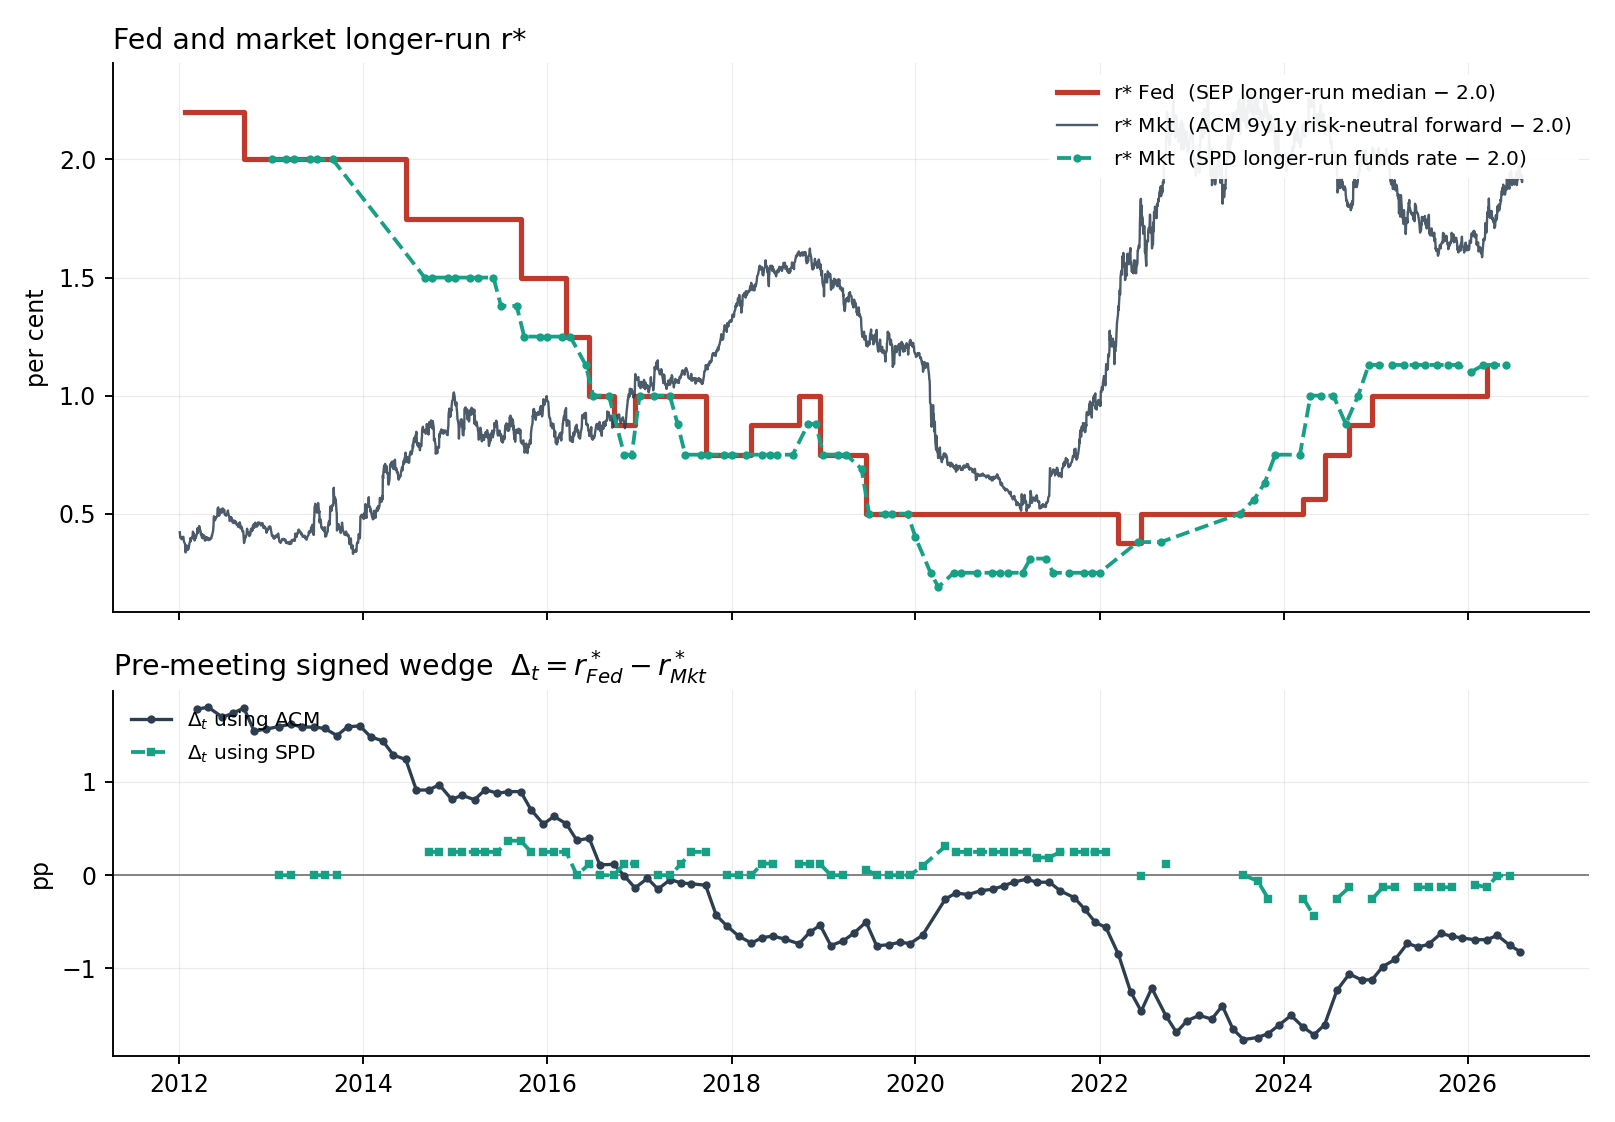
\includegraphics[width=0.645\textwidth]{figures/fig1_wedges.png}
    \end{center}
\end{frame}

% ------------------------------------------------------------------
\begin{frame}{What the gate killed}

\textbf{Check 1, $\pi^{*}$ dispersion: \kills, and completely.} All 594
participant longer-run PCE submissions across 36 meetings are exactly 2.0.
Maximum within-meeting standard deviation: $0.000000$. Meetings with any
dispersion: zero of 36. The SPD side is identical --- 2.0 in all 91 surveys,
including the twelve where the value is measured rather than assumed.

\vspace{0.6em}

$\rightarrow$ $\rstar$ is the longer-run dot minus a constant on \emph{both}
sides. The extraction is a relabelling. The design survives; the
\emph{real-rate framing does not}, and I would rather concede that than have
a referee find it.

\vspace{0.9em}

\textbf{Check 7, the SEP--SPD wedge: \kills.} Across 42 SEP meetings with a
same-month survey, mean $|$gap$|$ is 13.1bp, median 13.0bp, maximum 25.0bp.
Mercatus~[4] reported 42bp; on this panel it is tighter still. The survey
wedge has a variance of 0.028 because the two series are 94\% correlated.
There is no disagreement here to price.

\end{frame}

% ------------------------------------------------------------------
\begin{frame}{What the gate left standing}

\textbf{The ACM route \lives, with two flags.}

\vspace{0.5em}

\begin{center}
\small
\begin{tabular}{llcc}
\toprule
 & Check & SPD & ACM \\
\midrule
2 & var($\rstar_{Fed}$) share; corr($F,M$) & 49.9\%; $+0.94$ & 50.3\%; $\mathbf{-0.60}$ \\
3 & $R^{2}$ of $\Delta$ on each side alone & 0.03 / 0.03 & \textcolor{killred}{0.80 / 0.80} \\
5 & corr($\mathrm{d}\rstar_{Fed}, \mathrm{d}\rstar_{Mkt}$) & $+0.60$ & $-0.14$ \\
6 & AR(1) $\rho$ of $\Delta_t$ & $+0.85$ & \textcolor{killred}{$+0.98$} \\
\bottomrule
\end{tabular}
\end{center}

\vspace{0.55em}

\textbf{Where the variation comes from.} The ACM wedge has 38 times the
variance of the survey wedge, because market pricing moves \emph{against} the
SEP. That negative correlation is the entire source of identification.

\vspace{0.5em}

\textbf{Flag one.} Because $F$ and $M$ are negatively correlated, either one
alone explains 80\% of $\Delta$ --- not the degenerate case check~3 was
written to catch, but it makes the horse race mandatory.

\vspace{0.5em}

\textbf{Flag two, and it binds.} The SEP longer-run median \emph{changed 19
times in fourteen years}. Effective $N$ is 19, not 116.

\end{frame}

% ------------------------------------------------------------------
\begin{frame}{The result}

\textbf{Announcement-window response to the pre-meeting wedge}, bp per pp,
two-day window, 116 meetings, HAC(4).

\vspace{0.5em}

\begin{center}
\small
\begin{tabular}{lccc}
\toprule
Maturity & Total yield & Risk-neutral & Term premium \\
\midrule
2y  & $+2.25$ \; $(2.57)$ & $+1.46$ \; $(2.53)$ & $+0.79$ \; $(1.25)$ \\
5y  & $+3.34$ \; $(4.06)$ & $+1.72$ \; $(2.71)$ & $\mathbf{+1.62}$ \; $(3.21)$ \\
10y & $+3.14$ \; $(4.18)$ & $+1.49$ \; $(2.84)$ & $\mathbf{+1.65}$ \; $(2.52)$ \\
\bottomrule
\end{tabular}
\end{center}

\vspace{0.8em}

\textbf{Sign.} When the Fed sits above what the market is pricing, yields
rise into the window. The market moves toward the Fed. That is
Hillenbrand's channel and the risk-neutral column is its predicted signature
--- confirmation, not news.

\vspace{0.6em}

\textbf{The new column is the third one.} At 10y the premium response is
slightly larger than the expectations response. The SPD wedge gives nothing
anywhere, at any maturity, on any component.

\end{frame}

% ------------------------------------------------------------------
\begin{frame}{Before believing it: is it a free parameter of the construction?}

\textbf{The worry.} The wedge is built from the ACM risk-neutral curve at
$t-1$ and the regressand is the change in the same curve from $t-1$ to
$t+1$. ACM fits a \emph{stationary} VAR to yield principal components, which
mechanically produces a negative level-on-change relationship. The
regression could be pure mean reversion in the ACM state vector with no
announcement content at all.

\vspace{0.7em}

\textbf{The test.} Run the identical regression on every non-FOMC trading
day in the sample --- 3,513 of them.

\vspace{0.5em}

\begin{center}
\small
\begin{tabular}{lcc}
\toprule
10y component & FOMC days ($n=114$) & non-FOMC days ($n=3{,}513$) \\
\midrule
Total yield    & $+3.20$ \; $(4.32)$ & $-0.18$ \; $(-1.02)$ \\
Risk-neutral   & $+1.47$ \; $(2.75)$ & $-0.01$ \; $(-0.08)$ \\
Term premium   & $+1.73$ \; $(2.63)$ & $-0.17$ \; $(-1.04)$ \\
\bottomrule
\end{tabular}
\end{center}

\end{frame}

% ------------------------------------------------------------------
\begin{frame}{The same regression, run on 3,513 ordinary days}
    \begin{center}
        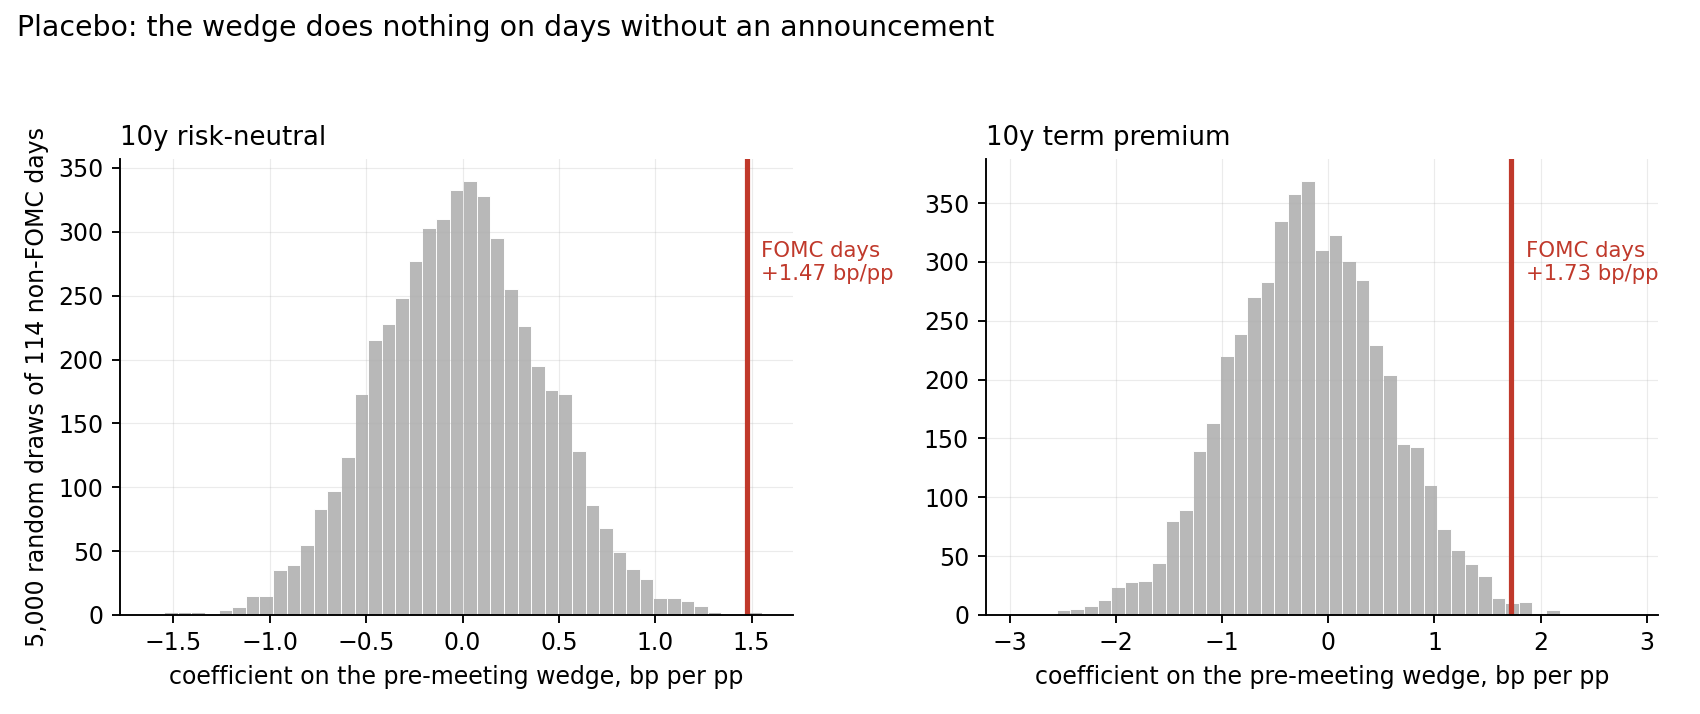
\includegraphics[width=0.88\textwidth]{figures/fig3_placebo.png}
    \end{center}
\end{frame}

% ------------------------------------------------------------------
\begin{frame}{Where it breaks}

\textbf{Inference.} Moving-block bootstrap, block length eight, roughly one
year of meetings. The risk-neutral coefficient gives $[+0.34, +3.01]$ and
excludes zero. The term premium gives $[-0.11, +2.57]$ and
\textcolor{killred}{includes zero}. The effect is also purely a
\emph{level} effect --- the change in the wedge since the previous meeting
predicts nothing, which is check~6 biting.

\vspace{0.7em}

\textbf{Subsamples, and this is the real problem.}

\begin{center}
\small
\begin{tabular}{lccc}
\toprule
10y & Total & Risk-neutral & Term premium \\
\midrule
2012--2015, ZLB              & $+5.44$ \; $(2.01)$ & $-0.48$ \; $(-0.24)$ & $\mathbf{+5.92}$ \; $(2.08)$ \\
2016--2019, normalisation    & $+0.22$ \; $(0.09)$ & $-0.80$ \; $(-0.44)$ & $+1.02$ \; $(0.76)$ \\
2020--2026, pandemic on      & $+6.71$ \; $(2.94)$ & $\mathbf{+5.07}$ \; $(4.00)$ & $+1.64$ \; $(0.86)$ \\
\bottomrule
\end{tabular}
\end{center}

\vspace{0.7em}

$\rightarrow$ The pooled headline averages two non-overlapping episodes. The
premium effect is a ZLB phenomenon; the expectations effect is a post-2020
phenomenon; the middle four years are null on everything.

\end{frame}

% ------------------------------------------------------------------
\begin{frame}{One thing that got stronger, not weaker}

\textbf{The premium response is not a by-product of the expectations move.}
Conditioning on the announcement's own near-term policy surprise --- the
cleanest available proxy being the window change in the 1y and 2y
risk-neutral rates --- the 10y term-premium coefficient \emph{rises}.

\vspace{0.6em}

\begin{center}
\small
\begin{tabular}{lccc}
\toprule
Specification & $b$ & $t$ & $R^{2}$ \\
\midrule
$\mathrm{d}TP^{(10)} \sim \Delta$                                 & $+1.65$ & $2.52$ & $0.039$ \\
$\mathrm{d}TP^{(10)} \sim \Delta + \mathrm{d}rn^{(1)}$            & $+2.23$ & $3.48$ & $0.175$ \\
$\mathrm{d}TP^{(10)} \sim \Delta + \mathrm{d}rn^{(1)} + \mathrm{d}rn^{(2)}$ & $+2.17$ & $3.55$ & $0.177$ \\
\bottomrule
\end{tabular}
\end{center}

\vspace{0.9em}

\textbf{And the sign of the wedge is what prices, not its size.} The absolute
wedge gives nothing. Split by direction, the term premium responds
\emph{only} when the Fed sits above the market ($+2.99$, $t = 2.50$; the other
side is a clean zero) and the risk-neutral component responds \emph{only}
when the Fed sits below ($-4.04$, $t = -3.96$). Two directions, two
components. That is either the most interesting thing here or the same
regime split of the previous slide seen twice, since 2012--2015 is a
Fed-above period and 2020--2026 is a Fed-below period.

\end{frame}

% ------------------------------------------------------------------
\begin{frame}{Maturity signature}
    \begin{center}
        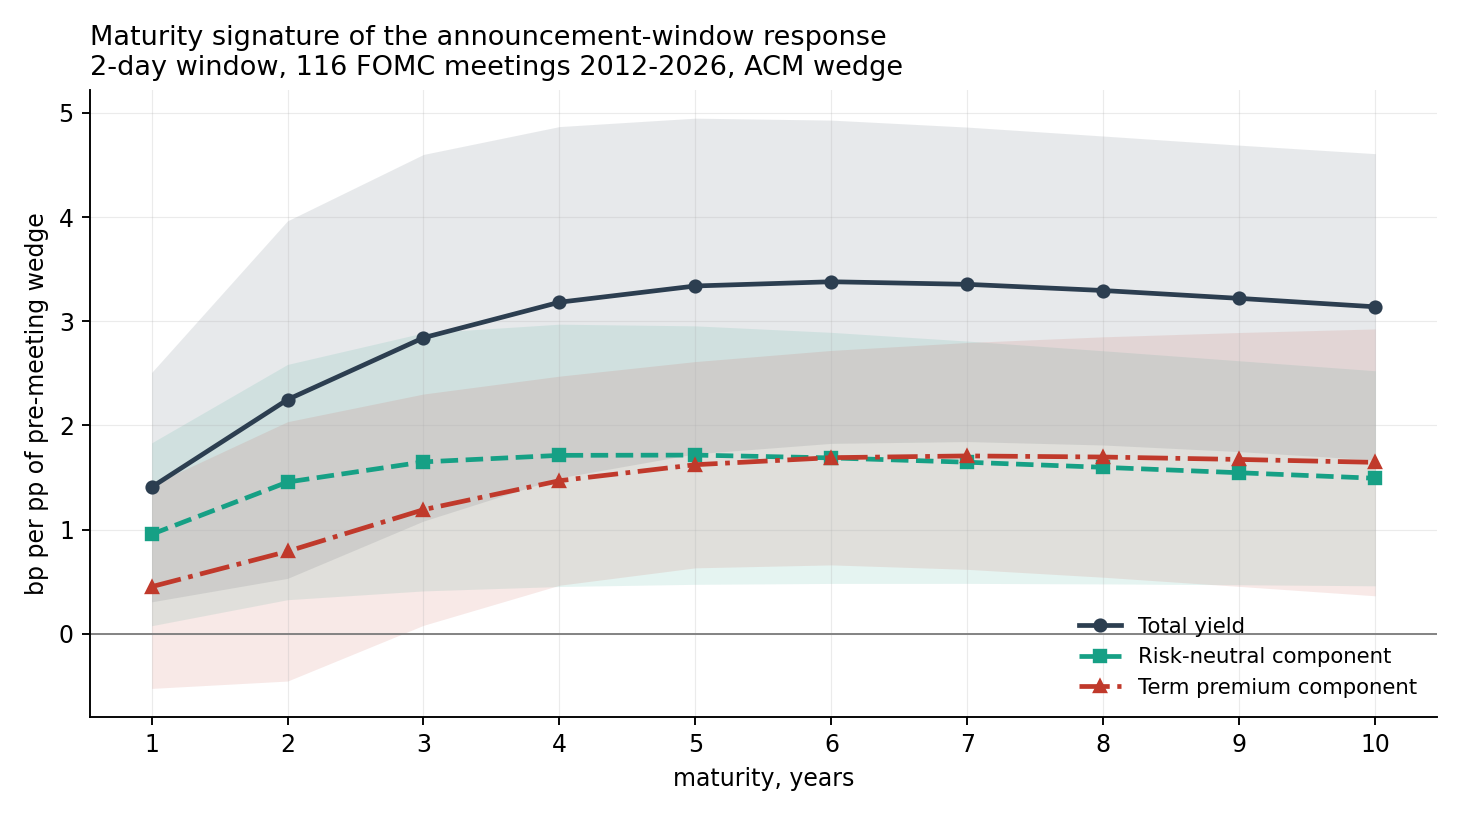
\includegraphics[width=0.72\textwidth]{figures/fig2_maturity.png}
    \end{center}
    \textbf{Neither profile.} An endpoint shock loads flat at one, a cyclical
    shock decays at $1/n$. Both components trace a hump peaking at 5--7y.
\end{frame}

% ------------------------------------------------------------------
\begin{frame}{What I would like to ask you}

\textbf{One. The regime split.} A premium effect that lives only at the ZLB
and an expectations effect that lives only after 2020 --- is that two
mechanisms or one badly specified one? Everything else is downstream of this,
and more robustness on the pooled sample does not address it.

\vspace{0.6em}

\textbf{Two. The Cieslak--Povala cycle.} Does it still contain $\rstar$
variation, and would an external $\rstar$ measure change the risk-premium
factor? Hillenbrand dismisses the risk-premium channel as unlikely to explain
the \emph{majority} of the decline, which is not the same as zero.

\vspace{0.6em}

\textbf{Three. Is anyone working on the premium component of the
announcement-window move?} Benigno's Substack in early August links
hall-of-mirrors to Hillenbrand and to a Lustig extension, and notes that
competing explanations imply different maturity profiles.

\vspace{0.6em}

\textbf{Four, a construction question.} The whole premium result is one
model's term premium, and ACM assumes a constant endpoint while the wedge is
a statement about the endpoint. Is Kim--Wright the right adversarial test, or
does its survey input make the comparison circular?

\end{frame}

% ------------------------------------------------------------------
\begin{frame}{Where this leaves things}

\textbf{Established.} The pre-meeting wedge moves announcement-window yields;
the relationship is absent on 3,513 non-announcement days and sits above
99.9\% of 5,000 randomised placebo samples; the risk-neutral coefficient
survives block-bootstrap inference. Hillenbrand's prediction holds on this
construction.

\vspace{0.6em}

\textbf{Not established.} The term-premium coefficient --- the actual
contribution --- is positive and HAC-significant, but its bootstrap interval
includes zero, it is entirely a 2012--2015 phenomenon, and it exists only
with the pricing-based wedge. Suggestive. Not a result.

\vspace{0.6em}

\textbf{Dead.} The SEP--SPD wedge as a Fed-versus-market object. The claim to
be measuring \emph{real}-rate disagreement.

\vspace{0.6em}

\textbf{Next.} Resolve the regime split; bring in a second term-premium model;
move the Fed side from the median, which changed 19 times, to the
cross-sectional dispersion, which takes 49 distinct values and is not near a
unit root.

\end{frame}

% ------------------------------------------------------------------
\begin{frame}{References}
\footnotesize
\begin{thebibliography}{9}
\bibitem{rw} Rungcharoenkitkul, P. and F. Winkler (2026). ``The Natural Rate
of Interest Through a Hall of Mirrors.'' \emph{Journal of Monetary
Economics} 157, 103858.
\bibitem{hb} Hillenbrand, S. (2025). ``The Fed and the Secular Decline in
Interest Rates.'' \emph{Review of Financial Studies} 38(4), 981--1013.
\bibitem{acm} Adrian, T., R. Crump and E. Moench (2013). ``Pricing the Term
Structure with Linear Regressions.'' \emph{Journal of Financial Economics}
110(1), 110--138.
\bibitem{merc} Mercatus Center (2025). Comparison of the SEP longer-run
median and the Survey of Primary Dealers, 2012--2025.
\bibitem{sr934} Cao, S., R. Crump, S. Eusepi and E. Moench (2020).
``Fundamental Disagreement about Monetary Policy and the Term Structure of
Interest Rates.'' Federal Reserve Bank of New York Staff Report 934.
\end{thebibliography}
\end{frame}

% ------------------------------------------------------------------
\appendix

\begin{frame}[noframenumbering]{Appendix: the horse race}

\textbf{Entering the two sides separately} instead of imposing the $-1$
coefficient the wedge assumes, 10y, two-day window.

\begin{center}
\small
\begin{tabular}{lccccc}
\toprule
 & Wedge & Mkt alone & Fed alone & Both (Fed / Mkt) & $b_F = -b_M$ \\
\midrule
Total        & $+3.14$ & $-4.59$ & $+5.07$ & $+3.27$ / $-3.00$ & $p = 0.935$ \\
Risk-neutral & $+1.49$ & $-2.59$ & $+2.07$ & $+0.71$ / $-2.28$ & $p = 0.363$ \\
Term premium & $+1.65$ & $-2.00$ & $+3.00$ & $+2.57$ / $-0.72$ & $p = 0.483$ \\
\bottomrule
\end{tabular}
\end{center}

\vspace{0.7em}

\textbf{The restriction is never rejected} --- the data are content to be
described by a single signed wedge. But the unrestricted coefficients say
something the wedge hides: the risk-neutral response loads on the
\emph{market} side and the premium response loads on the \emph{Fed} side.
The two components are answering different halves of the gap.

\end{frame}

\begin{frame}[noframenumbering]{Appendix: effective sample size and the fallback}

\textbf{The median.} 57 SEP meetings, 12 distinct values of the longer-run
$\rstar$, 19 meetings at which it changed, longest run without a change ten
meetings. AR(1) $\rho \approx 1$.

\vspace{0.7em}

\textbf{The fallback.} Cross-sectional dispersion of the same panel: mean
standard deviation 0.304, range $[0.217, 0.461]$, \emph{49 distinct values
over 57 meetings}, AR(1) $\rho = 0.803$.

\vspace{0.7em}

$\rightarrow$ Roughly 2.5 times the identifying variation, and not near a unit
root. If the median route stalls this is the better-powered object, and it
has its own asset-pricing interpretation via SR 934~[5].

\vspace{0.9em}

\textbf{Randomisation detail.} 5,000 draws of 114 random non-FOMC days.
Observed 10y risk-neutral coefficient sits at the 99.9th percentile
($p = 0.002$); term premium at the 99.4th ($p = 0.012$); total yield above
all 5,000 draws.

\end{frame}

\end{document}
